
\section{Sphärische Trigonometrie}
\rhead{Sphärische Trigonometrie}

\subsection{Das Kugeldreieck}
Damit man die Definition des Kugeldreiecks versteht, müssen wir zuerst Begriffe wie Grosskreisebene und Grosskreisbögen verstehen.
\index{Grosskreis}%
\index{Grosskreisebene}%
\index{Grosskreisbogen}%
Ein Grosskreis ist ein grösstmöglicher Kreis auf einer Kugel\-ober\-fläche.
Sein Mittelpunkt fällt immer mit dem Mittelpunkt der Kugel zusammen
und ein Schnitt auf dem Großkreis teilt die Kugel in jedem Fall in
zwei gleich grosse Hälften.
Da es unendlich viele Möglichkeiten gibt, eine Kugel so zu zerschneiden, dass die Schnittebene den Kugelmittelpunkt trifft, gibt es auch unendlich viele Grosskreise.
Grosskreisbögen sind die kürzesten Verbindungslinien zwischen zwei Punkten auf der Kugel.

Da die Länge der Grosskreisbögen wegen der Abhängigkeit vom Kugelradius ungeeignet ist, wird die Grösse einer Seite mit dem zugehörigen Mittelpunktwinkel des Grosskreisbogens angegeben. 
Laut dieser Definition ist die Seite $c$ der Winkel $AMB$, wobei der Punkt $M$ die Erdmitte ist.

Man kann bei Kugeldreiecken nicht so einfach unterscheiden, was Innen oder Aussen ist. 
Wenn man drei Eckpunkte miteinander verbindet, ergeben sich immer 16 Kugeldreiecke. 

Werden drei voneinander verschiedene Punkte, die sich nicht auf
derselben Grosskreisebene befinden, mit Grosskreisbögen verbunden
werden, so entsteht ein Kugeldreieck $ABC$.
Für ein Kugel\-drei\-eck gilt, dass die Summe der drei Seiten kleiner
als $3\pi$ aber grösser als 0 ist.
$A$, $B$ und $C$ sind die Ecken des Dreiecks und dessen Seiten sind die Grosskreisbögen zwischen den Eckpunkten (siehe Abbildung \ref{kugel}). 

\begin{figure}
	\begin{center}
		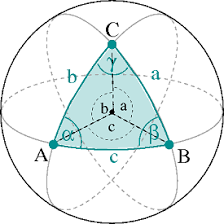
\includegraphics[width=3.5cm]{papers/nav/bilder/kugel1.png}
		\caption[Das Kugeldreieck]{Das Kugeldreieck}
		\label{kugel}
	\end{center}
	
\end{figure}

\subsection{Rechtwinkliges Dreieck und rechtseitiges Dreieck}
In der sphärischen Trigonometrie gibt es eine Symmetrie zwischen Seiten und Winkeln, also zu jedem Satz über Seiten und Winkel gibt es einen entsprechenden Satz, mit dem man Winkel durch Seiten und Seiten durch Winkel ersetzt hat.

Wie auch im ebenen Dreieck gibt es beim Kugeldreieck auch ein rechtwinkliges Kugeldreieck, bei dem ein Winkel $\frac{\pi}{2}$ ist. 
Ein rechtseitiges Dreieck gibt es jedoch nur beim Kugeldreieck, weil dort eine Seitenlänge $\frac{\pi}{2}$ lang sein muss, wie man in der Abbildung \ref{recht} sehen kann.

\begin{figure}
	
	\begin{center}
		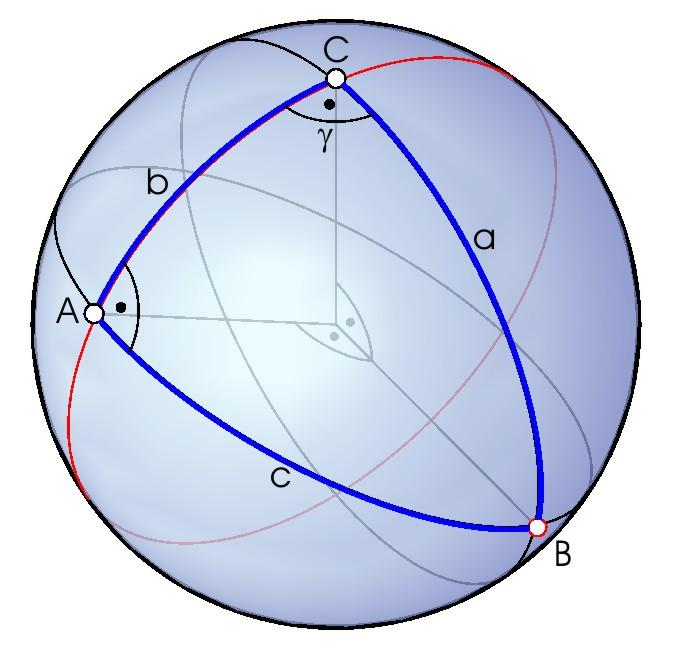
\includegraphics[width=5cm]{papers/nav/bilder/recht.jpg}
		\caption[Rechtseitiges und rechtwinkliges Kugeldreieck]{Rechtseitiges und rechtwinkliges Kugeldreieck}
		\label{recht}
	\end{center}	
\end{figure}

\subsection{Winkelsumme und Flächeninhalt}
\label{trigo}
\index{Winkelsumme}%
%\begin{figure} ----- Brauche das Bild eigentlich nicht!
	
%	\begin{center}
%		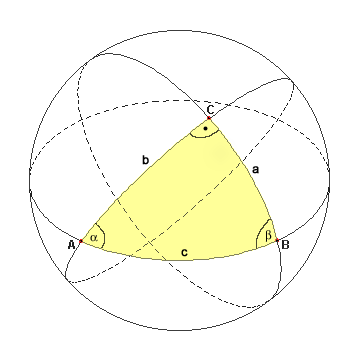
\includegraphics[width=8cm]{papers/nav/bilder/kugel2.png}
%		\caption[Winkelangabe im Kugeldreieck]{Winkelangabe im Kugeldreieck}
%	\end{center}	
%\end{figure}


Die Winkel eines Kugeldreiecks sind die, welche die Halbtangenten in den Eckpunkten einschliessen. 
Für die Summe der Innenwinkel gilt
\begin{align}
	\alpha+\beta+\gamma &= \frac{F}{r^2} + \pi \quad \text{und} \quad \alpha+\beta+\gamma > \pi, \nonumber
\end{align}
wobei $F$ der Flächeninhalt des Kugeldreiecks ist.
\subsubsection{Sphärischer Exzess}
\index{sphärischer Exzess}%
\index{Exzess, sphärischer}%
Der sphärische Exzess
\begin{align}
	\epsilon = \alpha+\beta+\gamma - \pi \nonumber
\end{align}  
beschreibt die Abweichung der Innenwinkelsumme von $\pi$ und ist proportional zum Flächeninhalt des Kugeldreiecks.
\index{Flächeninhalt}%

\subsubsection{Flächeninnhalt}
Mithilfe des Radius $r$ und dem sphärischen Exzess $\epsilon$ gilt für den Flächeninhalt 
\[ F=\frac{\pi \cdot r^2}{\frac{\pi}{2}} \cdot \epsilon = 2 \cdot r^2 \cdot \epsilon.\]

In diesem Kapitel sind keine Begründungen für die erhaltenen Resultate im Abschnitt \ref{trigo} zu erwarten und können in der Referenz \cite{nav:winkel} nachgeschlagen werden.
\subsection{Seiten und Winkelberechnung}
Es gibt in der sphärischen Trigonometrie eigentlich gar keinen Satz des Pythagoras, wie man ihn aus der zweidimensionalen Geometrie kennt.
\index{Pythagoras}%
Es gibt aber einen Satz, der alle drei Seiten eines rechtwinkligen Kugeldreiecks in eine Beziehung bringt. Dieser Satz gilt jedoch nicht für das rechtseitige Kugeldreieck.
Die Approximation im nächsten Abschnitt wird erklären, warum man dies als eine Form des Satzes des Pythagoras sehen kann.
Es gilt nämlich:
\begin{align}
	\cos c = \cos a \cdot \cos b \quad \text{wenn}  \nonumber &
	\quad \alpha = \frac{\pi}{2}. \nonumber
\end{align}

\subsubsection{Approximation von kleinen Dreiecken}
Die Sätze in der ebenen Trigonometrie sind eigentlich Approximationen der sphärischen Trigonometrie.
So ist der Sinussatz in der Ebene nur eine Annäherung des sphärischen Sinussatzes. Das Gleiche gilt für den Kosinussatz und dem Satz des Pythagoras.
So kann mit dem Taylorpolynom 2. Grades den Sinus und den Kosinus vom Sphärischen in die Ebene approximieren: 
\begin{align}
	\sin(a) &\approx a \nonumber \intertext{und}
	\cos(a)&\approx 1-\frac{a^2}{2}.\nonumber
\end{align}
Es gibt ebenfalls folgende Approximierung der Seiten von der Sphäre in die Ebene:
\begin{align}
	a &\approx \sin(a) \nonumber \intertext{und}
	\frac{a^2}{2} &\approx 1-\cos(a). \nonumber
\end{align}
Die Korrespondenzen zwischen der ebenen und sphärischen Trigonometrie werden in den kommenden Abschnitten erläutert.

\subsubsection{Sphärischer Satz des Pythagoras}
Die Korrespondenz \[ a^2 \approx 1- \cos(a)\] liefert unter anderem einen entsprechenden Satz des Pythagoras, nämlich

\begin{align*}
	\cos(a)\cdot \cos(b) &= \cos(c),  \\
	\bigg[1-\frac{a^2}{2}\bigg] \cdot \bigg[1-\frac{b^2}{2}\bigg] &= 1-\frac{c^2}{2}. 
	\intertext{Höhere Potenzen vernachlässigen:} 
	\xcancel{1}- \frac{a^2}{2} - \frac{b^2}{2} + \xcancel{\frac{a^2b^2}{4}}&= \xcancel{1}- \frac{c^2}{2}  \\
	-a^2-b^2 &=-c^2\\
	a^2+b^2&=c^2.
\end{align*}
Dies ist der wohlbekannte ebene Satz des Pythagoras.
\index{Pythagoras, Satz des}%
\index{Satz!von Pythagoras}%

\subsubsection{Sphärischer Sinussatz}
Den sphärischen Sinussatz 
\begin{align}
	\frac{\sin (a)}{\sin (\alpha)} =\frac{\sin (b)}{\sin (\beta)} = \frac{\sin (c)}{\sin (\gamma)} \nonumber
\end{align}
kann man ebenfalls mit der Korrespondenz \[a \approx \sin(a) \] zum entsprechenden ebenen Sinussatz \[\frac{a}{\sin (\alpha)} =\frac{b}{\sin (\beta)} = \frac{c}{\sin (\gamma)}\] approximieren.


\subsubsection{Sphärische Kosinussätze}
In der sphärischen Trigonometrie gibt es den Seitenkosinussatz
\index{Seitenkosinussatz}%
\begin{align}
	\cos \ a = \cos b \cdot \cos c + \sin b \cdot \sin c \cdot \cos \alpha \nonumber
\end{align} %Seitenkosinussatz
und den Winkelkosinussatz
\index{Winkelkosinussatz}%
\begin{align}
	\cos \gamma = -\cos \alpha \cdot \cos \beta + \sin \alpha \cdot \sin \beta \cdot \cos c, \nonumber
\end{align} der nur in der sphärischen Trigonometrie vorhanden ist.

Analog gibt es auch beim Seitenkosinussatz eine Korrespondenz zu \[ a^2 \leftrightarrow 1-\cos(a),\] die den ebenen Kosinussatz herleiten lässt, nämlich
\begin{align}
	\cos(a)&= \cos(b)\cdot \cos(c) + \sin(b) \cdot \sin(c)\cdot \cos(\alpha)  \\
	1-\frac{a^2}{2} &= \bigg[1-\frac{b^2}{2}\bigg]\bigg[1-\frac{c^2}{2}\bigg]+bc\cdot\cos(\alpha). \intertext{Höhere Potenzen vernachlässigen:}
	\xcancel{1}-\frac{a^2}{2} &= \xcancel{1}-\frac{b^2}{2}-\frac{c^2}{2} \xcancel{+\frac{b^2c^2}{4}}+bc \cdot \cos(\alpha)\\
	a^2&=b^2+c^2-2bc \cdot \cos(\alpha).
\end{align}


 
